
% Also note that the "draftcls" or "draftclsnofoot", not "draft", option
% should be used if it is desired that the figures are to be displayed in
% draft mode.
%
\documentclass[draftcls, onecolumn, 11pt]{IEEEtran}
%\documentclass[conference, twocolumn]{IEEEtran}

%\usepackage[latin1]{inputenc} % Latin1
\usepackage[utf8]{inputenc} 	% UTF-8

%\usepackage{amsmath,amsthm}
\usepackage{amssymb}
%\usepackage{amsfonts}
\usepackage{bbm} % For indicator function
%\usepackage{breeq}
\usepackage{graphicx}
\usepackage{color,psfrag}


% Dashed arrow and control the size of the braces due to underbrace
\usepackage{MnSymbol}
%\graphicspath{{./figures/}}

%Strike out the sentence
\usepackage[normalem]{ulem}

\usepackage{tikz}
\usepackage{siunitx}
\usepackage{makecell}

% Notations and symbols 
\newcommand{\sub}[1]{_{\text{#1}}}
\newcommand{\e}[2]{{\mathbb E}_{#1}\left[ #2 \right]}



\newcommand{\rs}{R\sub{s}}
\newcommand{\ers}{\e{}{\rs}}
\newcommand{\npu}{\Delta\sigma^2}
%\newcommand{\snrrcvd}{\gamma\sub{rcvd}}
\newcommand{\snrrcvd}{\text{SNR}}
\newcommand{\pc}{\text{P}\sub{c}}
\newcommand{\pcd}{\bar{\text{P}}\sub{c}}
\newcommand{\pd}{\text{P}\sub{d}}
\newcommand{\pdd}{\bar{\text{P}}\sub{d}}
\newcommand{\pf}{\text{P}\sub{fa}}
\newcommand{\hp}{h\sub{p}}
\newcommand{\hpo}{h\sub{p,1}}
\newcommand{\hpt}{h\sub{p,2}}
\newcommand{\hs}{h\sub{s}}
\newcommand{\fsam}{f\sub{s}}
\newcommand{\test}{\tau\sub{est}}
\newcommand{\tsen}{\tau\sub{sen}}

% Draw something blocks or ovelap
\usepackage{tikz}
\usepackage{siunitx}
\usepackage{cite} % Combining multiple citations

\usepackage{url}

% Subfigures
\ifCLASSOPTIONcompsoc
\usepackage[caption=false,font=normalsize,labelfont=sf,textfont=sf]{subfig}
\else
\usepackage[caption=false,font=footnotesize]{subfig}
\fi


% Metadata
\usepackage[final=true]{hyperref}
%%\hypersetup{
%	pdfauthor = {Ankit Kaushik et al.},
%	pdftitle = {IEEE Communications Magazine 2015},
%	pdfsubject = {IEEE Communications Magazine 2015},
%	pdfcreator = {PDFLaTeX with hyperref package},
%	pdfproducer = {PDFLaTeX}
%	hidelinks = {true}
%}


% Used to break the theorems, proof between the columns
\allowdisplaybreaks

%used to equalize the last pages
%\usepackage{flushend}

\begin{document}
%
\title{Cognitive Small Cell Deployment for Next Generation Wireless Systems}
\author{\IEEEauthorblockN{Ankit Kaushik\IEEEauthorrefmark{1}, Shree Krishna Sharma\IEEEauthorrefmark{2}, Holger Jaekel\IEEEauthorrefmark{1}, Friedrich Jondral\IEEEauthorrefmark{1}} \\
\IEEEauthorblockA{\IEEEauthorrefmark{1}Communications Engineering Lab, Karlsruhe Institute of Technology (KIT), Germany} \\ 
%\{ankit.kaushik, Holger.Jaekel, friedrich.jondral\}@kit.edu \\
\IEEEauthorblockA{\IEEEauthorrefmark{2}SnT - securityandtrust.lu, University of Luxembourg, Luxembourg} \\ 
%\{shree.sharma\}@uni.lu
Contact Information: Ankit.Kaushik@kit.edu
}

%\IEEEaftertitletext{Contact Information: Ankit.kaushik@kit.edu}
%\author{Ankit Kaushik, Holger Jaekel, Friedrich Jondral \\ Communications Engineering Lab \\ Karlsruhe Institute of Technology (KIT) \\ \{\href{mailto:Ankit.Kaushik@kit.edu}{Ankit.Kaushik},
%\href{mailto:Holger.Jaekel@kit.edu}{Holger.Jaekel}, \href{mailto:Friedrich.Jondral@kit.edu}{Friedrich.Jondral}\}@kit.edu
%}

% make the title area
\maketitle
\thispagestyle{empty}
\pagestyle{empty}

\begin{abstract}
The upcoming decade is about to witness a tremendous growth in the popularity of smart devices. 
%Integrating these enormous number of devices in the existing network is the biggest challenge faced by the community. 
The integration of these enormous number of devices in the network is the biggest challenge currently faced by the wireless community. To encounter this, ultra-densification and spectrum extension are envisioned as the paramount solutions. Given the constraints in deployment costs and the available spectrum, these solutions appear to be indomitable. In order to breakthrough these bottlenecks, we propose a deployment-centric viewpoint to the concept of Cognitive Small Cell (CSC) that jointly resolves the issues with small cell and spectrum scarcity. In this article, we highlight the significant steps necessary for the deployment of this notion in (Fifth-Generation) 5G networks. Another interesting element in our study is the introduction of a novel model that facilitates the feasibility of the opportunistic access for the CSC. Based on this model, we characterize the true performance of interweave and underlay cognitive systems. 
\end{abstract}

%\subsection{Background}
%\begin{itemize}
%\item Current status of the Cognitive Radio -- state of the art includes IEEE standards and LSA. However, does these business models portrays Mitola's vision? 
%\item Models lacking deployment aspects -- assumptions are too strong to be considered for a deployment over a hardware.
%\item Spectrum scarcity in the 5G networks, Cognitive Small Cell (CSC) is emerging as a new use case to cognitive radio. Cognitive radio has found its niche in the 5G. The requirements for the 5G have been laid: (i) the areal capacity in $\SI{}{bits/m^2}$ must roughly increase by ($\ge 1000 \times$) compare to 4G, (ii) low latency $\approx \SI{1}{ms}$ and, (iii) energy and cost efficient small cells. For the demand stated, ultra-densification and spectrum extension can contribute a large portion to the required areal capacity. Cognitive Small Cells can be seen as new use case to the cognitive radio. According to which the deployment leads to densification, and indoor access between the Here we try to motivate the benefits of the deploying Cognitive Small Cell (CSC). 
%\item Deployment Scenario for CSC
 	%\begin{itemize}
	%\item Do we really have spectrum scarcity or its inefficient use is making it scare. This debate will depict the future of next generation wireless systems. Spectrum usage for the CSC ($<$ \SI{6}{Hz} and $>$ \SI{6}{Hz}). Beyond $\SI{6}{GHz}$, penetration is reduced, thus to sustain coverage CSC has to operated at higher power. This issue is resolved for spectrum below $\SI{6}{GHz}$,  
	%\item Indoor and outdoor antenna
	%\end{itemize}	
%\item Cognitive Small Cell (CSC) as interweave system
%\item Cognitive Small Cell (CSC) as underlay system
%\item How software defined architecture could harness the future of cognitive radio?  
%\item Research Challenges
%\end{itemize}

%%%%%%%%%%%%%%%%%%%%%%%%%%%%%%%%%%%%%%%%%%%%%%%%%%%%%%%%%%%%%%%%%%%%%%%%%%%%%%%%%%%%%%%%%
\section{Introduction and Motivation}
%%%%%%%%%%%%%%%%%%%%%%%%%%%%%%%%%%%%%%%%%%%%%%%%%%%%%%%%%%%%%%%%%%%%%%%%%%%%%%%%%%%%%%%%%
Since the invention of smart phones in 2007, the mobile traffic has proliferated tremendously. Following the market analysis of mobile traffic done by CISCO \cite{CISCO14}, it is evident that this trend prevails also in the future. It is a well-known fact that the state-of-art technologies (Multiple Input Multiple Output), waveforms (Orthogonal Frequency Division Multiplexing) and standards (Fourth-Generation (4G) -- LTE, WiMAX) are not capable of sustaining these demands in the upcoming decade. With this situation in hand, we are currently in the process of conceptualizing the requirements for the next generation wireless systems. Some of these requirements are: (i) areal capacity in $\SI{}{bits/sec/m^2}$ must increase by a factor of $1000$ compared to 4G, (ii) low latency of approximately \SI{1}{ms}, and, (iii) energy- and cost-efficient deployment \cite{Andrews14}.

In the recent past, Small Cells (SCs) have emerged as a potential solution for coverage and capacity enhancements in a network. An SC represents a low power station that ranges from $\SI{10}{m}$ to $\SI{100}{m}$, comparable to the size of a femtocell. The reduced transmit distance accomplished with the deployment of SCs enhances the link quality and aids spatial reuse \cite{Chander08}. 
%SC is particularly deployed in a indoor or outdoor environments, these include enterprise, shopping complex or residential \cite{SSF14}. 
As a result, ultra-densification via SCs is envisaged as the absolute paramount for the Fifth-Generation (5G) of wireless systems \cite{Andrews14}. 
The capacity, however, increases linearly with the number of SCs, hence, it is implausible to procure the factor of $1000$ in the areal capacity with ultra-densification alone.  
Additionally, backhaul deployment and operation of these substantial number of SCs are cost- and energy-intensive for the mobile operator.  
Complementing the link quality, the spectrum procures a large contribution to the areal capacity. Given the current situation of the spectrum allocated for mobile communications, an extension in the available spectrum is imperative. In this regard, we consider the classification for the spectrum extension as: 
%\begin{itemize}
(i) $\ge \SI{6}{GHz}$; 
(ii) $\le \SI{6}{GHz}$. 
%\end{itemize}
The prime objective of this sort of classification is to shift the focus on the propagation characteristics and the issues thereof.   

The spectrum beyond \SI{6}{GHz} largely entails the millimeter Wave (mmW), which is well-known for point-to-point communications. This range has been limited mainly to satellite or short range communications. Recently, it has been envisaged as a powerful source of spectrum for the 5G systems. However, in the present scenario, mmW technology is surmounted with key-challenges like propagation loss, low efficiency of Radio Frequency (RF) components such as power amplifiers, size of the antenna and link acquisition
%\footnote{It states the responsivness of the base station to the movements of MS.} 
that need to be addressed. On the contrary, features like adaptive-beamforming are key-enablers of this technology. % to mitigate the interference, thereby characterizing noise as the limiting factor. 
In order to illustrate its feasibility, different scenarios have come forward to harmonize mmW spectrum into 5G, such as short range communications inside SCs and wireless backhaul. 
%These scenarios are limited to PTP communications. 
Recently, Rappaport \textit{et al.} \cite{Rapp13} investigated the propagation issues at \SI{28}{GHz} and \SI{38}{GHz} bands, this, however, raises a bigger question on its ability to sustain the mobility in a wireless network. 
Therefore, to capture a deeper insight of its feasibility in 5G, it is essential to overcome the aforementioned challenges in the forthcoming future. 


The spectrum below $\SI{6}{GHz}$ is utilized mainly for terrestrial wireless communication. Due to the static allotment of licenses by the regulatory bodies in this range, it is currently on the verge of scarcity. Given the spectrum is used efficiently, it is feasible to surmount this scarcity, for instance by means of opportunistic access. In this context, Cognitive Radio (CR), a concept introduced by Mitola in 1999 \cite{Mitola99}, is a suitable candidate that enables secondary access to the underutilized spectrum. Devices operating on the CR principles require the capability of \textit{learning} and \textit{responding} to the changes in the environment. Although, in its original definition, CR embraces physical, medium access and application layers, in this article, we focus on the physical layer aspects. 

Over the past several years, CR has engaged a large expertise of people from research, industry and regulatory bodies. Thereof, CR has found its niche in varied applications such as wireless microphones in TV white space and satellite communication. Several organizations, mainly IEEE and European Telecommunication Standard Institute \cite{ETSI13} have taken the responsibility of standardizing the CR technology. The chronology of these events clearly indicates that this technology has evolved at a significant pace and has achieved a certain level of maturity in the last years. Hence, it is a rightful moment, where we should consolidate our efforts on dispositioning this technology in the 5G systems. 

Following the previous discussion, it is evident that spectrum extension and SCs are key-enablers for the 5G system. 
%Recently, ElSawy \textit{et al.} \cite{Elsawy13} have presented Cognitive Small Cell (CSC), a concept that fulfills the capacity demands of the future wireless networks. 
Motivated by this fact, we establish a concept of Cognitive Small Cell (CSC), a promising approach that jointly enhances the SC deployment and the efficient usage of the spectrum below \SI{6}{GHz}. The notion of CSC has been previously investigated by Elsawy \textit{et al.} \cite{Elsawy13}, where the authors primarily emphasized on the modelling techniques that illustrate the positioning of several CSCs inside the network. In the view of this, the performance analysis of the CSC was constricted mainly to network abstraction. In this article, we provide a deployment-centric viewpoint to ensure a successful integration of CSCs in the 5G network. Consequently, by considering different CR paradigms to enable secondary usage of the licensed spectrum, we illustrate a deeper comprehension of the concept. %, thereby, making it accessible to 5G systems. 
To strengthen our understanding of CSC, we demonstrate the feasibility of the respective paradigms by means of hardware implementations.
%Pertaining to the deployment, we analyze the true performance of the CSC as a CR application for the mentioned paradigms.  

The subsequent sections of this article are organized as follows: Section \ref{sec:depl} proposes a viable disposition of CSC in a 5G network. Section \ref{sec:DR} presents the deployment insights for the CSC. Particularly, a deployment model to characterize the true performance of the CSC is proposed. Section \ref{sec:para_i} and Section \ref{sec:para_u} evaluate the performance of CSC as interweave and underlay paradigms based on the deployment model, respectively. Section \ref{sec:r_cha} briefly discusses the open challenges involved. Finally, Section \ref{sec:conc} concludes the article. 
%In order to consider ultra-densification, it is necessary to apply the wisdom "deploy wherever necessary". According to which it is necessary to correlate the SC deployment with the traffic demands rather then engulfing the entire spatial region. 
%However, these such deployment of will be faced with the following challenges: (i) Capacity is still a limited, (ii) capital and operation expenditure SC Cost driven and (ii) Capital expenditure (CAPEX) with the deployment of backhaul and the Operation Expenditure (OPEX) and (ii) co-tier capacity is limited by the co-tier and cross-inter interference. 
%However, before proceeding with the deployment, it is necessary to 
%However, ultra-densification will face many challenges: most particularly, the cost of deploying the backhaul and operation costs. Still, ultra-densifcation solely cannot sustain the capacity demands for 5G. 
%To sustain the  intends to sustain the desired Quality of Experience (QoE).  
   
%A Cognitive Radio \cite{Mitola99} is a perception induced in wireless communications that endeavors efficient utilization of its resources, for instance energy and spectrum. For last one and a half decades, CR has engaged a large expertise of people from research, industry and regulatory bodies. Thus, evolved as a potential solution to address the problem of spectrum scarcity. This process has led to the formulation of different business models: IEEE standards and Licensed Shared Access (LSA).  
%This stalemate is greatly due to the mismatch in the way these two communities perceive the concept of Cognitive Radio. 
%Mobile operators deals mainly with scenarios that employ Licensed Shared Access (LSA) to the spectrum. 

%\subsubsection*{IEEE}
%IEEE working Groups mobilized with the responsibility of enabling unlicensed access in TV white space for the following standards: IEEE 802.11af, 802.22, 802.15.4m, 802.19.1 and DySPAN SC 1900.7. As a result of their efforts, the design specifications for the PHY and MAC can be procured as draft versions \cite{Sum13}. Recently, IEEE 802.11ax: High-Efficiency WLAN (HEW), a study group created for the next generation WLANs. Given the dense scenarios, the HEW intends to increase area throughput and improve interference coordination among the neighbouring APs.  

%\subsubsection*{License Shared Access}
%Proposed by ETSI \cite{ETSI13}, LSA is deemed to satisfy the spectral demands particularly for the cellular industry. According to the current version, a licensing agreement exists between the incumbent and licensee, which could last several months or years. During this window, the licensee is granted spectrum for its exclusive use. In order to endorse spectrum access in the network, it is necessary to include following entities in LSA framework: an LSA controller and a repository. The LSA controller certifies a fair trading of the spectrum among different secondary systems. Whereas the repository constitutes the frequency channels of the incumbents based on their geographical locations. The existent LSA framework portrays a static scenario, however its future versions are dynamic and intend to reduce the time duration for the shared access to a \SI{}{ms} scale. %The operator can consider a centralized or a decentralized system for these entities. This choice rather depends on its delay requirements. Though systems following decentralized approach experience low latency, but often require synchronization updates. This could possible threat to the performance for a large network.

%On the other side, researchers find these scenarios rather unattractive, thus are driven toward more dynamic use cases. The main focus is to characterize the performance of cognitive radio systems analytically, thereby paying less attention to the deployment scenarios. In this process of designing a system model, they tend to include assumptions that prohibit the implementation of these models on a real hardware. At this time, it is necessary to come up with new models or modify the existing models such that they can be considered in future for hardware deployment. %Apart from that, because these models differ from each another, it becomes rather impossible to consider them for a deployment. 
%Goldsmith \textit{et .al} \cite{Goldsmith09}


%Though these models have made the deployment plausible and increases spectral efficiency, however they are capable of nurturing the short term demands only. Considering the capacity demands for upcoming wireless systems, these models can only sustain short term targets. 

%It is envisaged that 80\% of the radio access will be indoor, i.e., enterprises, shopping complexes and residential areas \cite{Zukerman}, which forbids macro penetration. Thereby creating coverage holes in the network. Small cell\footnote{Here small cell is comparable or smaller than the size of a femtocell, that ranges from $\SI{10}{m}$ to $\SI{50}{m}$.} deployment has emerged as a vital solution that intends to uplift the coverage and sustain the desired Quality of Service (QoS). Given full frequency reuse in a multi-tier network, it becomes necessary to employ interference management protocols that suppress cross-tier and co-tier interference. Such networks are defined as Self-Organizing Networks (SON). 


%For an operator, such coordination techniques in SON result in higher spectral efficiency for the alloted spectrum, however, it doesn't suffice the capacity requirements for the future wireless systems. %One such way to fulfill this demand is through secondary access to the licensed spectrum. %Two system can co-exist only when seek separation in time, frequency, space and polarization. 
%Considering the spectrum access for the 5G, two scenarios are coming forward. The first scenario target spectrum beyond $\SI{6}{GHz}$, falling under the \SI{}{mm}-wave. Recently, Cognitive Small Cell (CSC), an application to cognitive radio, is envisioned as a feasible solution for 5G systems. CSCs are meant to be deployed in the network, that perform secondary access to the unused spectrum.   
%However, it is necessary the successful function of the licensed system. Small cell especially indoor scenarios are the prime candidate for such   


%This article presents three major aspects. The first section talks about the CSC scenario deployed as cognitive radio system. Second section consider the different paradigm for CSC, specially, how theses paradigms could pave the path towards its deployment. Finally, we demonstrate the preliminary investigation concerning CSC and discuss the future research challenges while deploying such a system on a hardware. 

%The article presents three major aspects:

%%%%%%%%%%%%%%%%%%%%%%%%%%%%%%%%%%%%%%%%%%%%%%%%%%%%%%%%%%%%%%%%%%%%%%%%%%%%%%%%%%%%%%%%%
\section{Disposition of CSC in 5G network} \label{sec:depl}
%%%%%%%%%%%%%%%%%%%%%%%%%%%%%%%%%%%%%%%%%%%%%%%%%%%%%%%%%%%%%%%%%%%%%%%%%%%%%%%%%%%%%%%%%
\begin{figure}[!t]
\centering
\includegraphics[width = 0.7 \columnwidth]{figures/Cellular_Scenario_CR6F}
\caption{An illustration of the CSC deployment in a 5G network.}
\label{fig:scenario}
\end{figure}
%In this section, we consider the deployment scenario for CSC. 
This section illustrates a comprehensive incorporation of CSC in a preliminary 5G architecture. From the market analysis, it has been depicted that $70\%$ of the data traffic is originated indoor \cite{Chander08}. In addition, a new range of wireless services, categorized as Internet of Things, will operate from indoor. Thus, the effects will be far more consequential if we consolidate these sources of data traffic by means of SCs deployment. In this regard, it is sensible to consider the residential and enterprise as the main deployment scenarios for the CSC, cf. \figurename~\ref{fig:scenario}. Except for a different coverage regime, the operating principles of these scenarios are analogous. 

\subsection*{Network Elements}
For the disposition of the CSC in the network, the following key elements are essential: a CSC-Base Station (CSC-BS), a Macro Cell-Base Station (MC-BS) and Mobile Stations (MSs), cf. \figurename~\ref{fig:scenario}. MSs are the devices either served by the MC-BS over a \textit{Direct Access} link or the CSC-BS over an \textit{Indirect Access} (IA) link. Furthermore, the MC-BS is connected to several CSC-BSs over a \textit{Wireless Backhaul} (WB) link. Although the MC-BS and the MS already exist in the conventional cellular architecture, to incorporate the opportunistic access inside the CSC, it is necessary to consider a functionality upgrade.

\subsection*{Spectrum Access}
In the proposed network architecture, the access to the spectrum is realized over the WB, the DA and the IA links, cf. \figurename~\ref{fig:scenario}. 
\begin{enumerate}
\item A WB is a 
%quasi-line of sight\footnote{It allows limited number of objects between the direct link.} 
point-to-point wireless link between the CSC-BS and MC-BS that relays the traffic generated from the CSC to the core network. Accounting the feasibility of ultra-dense CSC, the WB link presents a cost-effective and energy-efficient alternative to the mobile operator. 
With the limited infrastructure required for deployment, it accelerates installation and promotes scalability of the network. 
For the WB link, an exclusive spectrum for a longer duration is desired, hence, it is sensible to nominate a mmW band; alternatively, an exclusive band below \SI{6}{GHz} can be acquired using the principles of Licensed Shared Access \cite{ETSI13}. 
%These WB links encourage ultra-densification as they brings down the capital expenditure and offer scalability to the vendor. 

\item A DA link represents a direct access of the MS at the MC-BS over the allocated spectrum. Consequently, the spectrum access for this link is analogous to the one existing in the state-of-art wireless standards. 
\item The CSC elements (the CSC-BS and the MS) are responsible for executing secondary access to the licensed spectrum. The additional spectrum acquired is used for the communication between the CSC-BS and the MS over the IA link.
\end{enumerate} 
%Obviously, the preliminary information about the channels (center frequency and bandwidth, etc.) is made available to CSC-BS in the form of database. 
%Now, to execute the dynamic access to the unused spectrum, CSC-BS obeys the basic principles of CR: \textit{spectrum-awareness} and \textit{spectrum-exploitation}. This can be instantiated as follows: in the first step, the CSC-BS acquires the knowledge of unknown parameters for each channel present in the database. Those channels that sustain the sharing constraints are proceeded for the data transmission. 
%\begin{itemize}
%\item The CR possess the cell ID and provides provides the signalling to the MSs. 
%\item Understanding the traffic demand, it is important to not only just deploy cells, most important is to deploy small cells where demand exists. Indoor scenarios and hot spots are typical use cases.  
%\end{itemize}

\subsection*{Hardware Feasibility}
Here, we outline the main aspects that pertain to the hardware realizability of the CSC. For the CSC-BS, an antenna mount system consisting of an indoor and outdoor antenna is proposed. Whereby, the indoor antenna exploits the walls of the building to physically separate the indoor transmissions over the IA link, in this way, it curtails the interference to the primary system and neighbouring CSCs.
Whereas, the outdoor antenna secures a narrow beam transmission to enhance the link quality for the WB link. 

In order to illustrate rapid prototyping and realize cognitive functionality on a real hardware, Software Defined Radio (SDR) platform is a viable solution. SDR has played a vital role in the genesis of the CR \cite{Jondral05}. Taking this into account, we inherit the eminent features of SDR for the hardware deployment of CSC-BS and MS. Some of these include:
\begin{itemize}
%\item A multi-band system, supporting transmission or reception over several channels, is required to support data transmissions over non-contiguous channels via IA link. %In case the simultaneous transmission or reception is not feasible because of bandwidth limitation channels are sparsely located  
\item Multi-channel support -- To enable independent transmission or reception of non-contiguous channels over the WB and the IA link.
%\item Frequency translation from WB link to IA link, for instance \SI{2.3}{GHz} to \SI{28}{GHz}.
\item Real-time reconfigurability -- With activation of Primary Users (PUs), the hardware should be capable of reconfiguring its RF parameters with minimum latency. %This assures a seamless handover by restricting the switching time between two channels to a lower value. %This the CSC-SC and MSs capable to respond to a dynamic situation, for instance, discontinuation of transmission due to notification of an activity by the primary system.
%\item Multi-standard capability -- CSC-BS and MS must be robust to the physical and medium access, in case, secondary access to multiple primary systems is desired. 
\end{itemize} 
 
\subsection*{Network Compatibility}
Besides secondary access, CSC has to co-exist harmoniously with the other elements existing in the network. In this context, the network elements are embedded with additional functionality such as:
\begin{itemize}
\item The MS procures the control information (signalling and synchronization) over the IA link after connecting to the near-by CSC-BS.  
\item To sustain a logical placement of CSCs inside the network, the CSC employs S1 and X2 interfaces over the WB link. 
%Under this situation, the MC-BS, however, remains transparent to the additional spectrum acquired by the CSC over the IA link. 
%For the co-exisitence it is necessary to consider the co-existence of CSCs under the MC. 
\item For situations where several CSC-BSs co-exist under a MC-BS, operations like seamless cross-tier and co-tier mobility constitute a challenging task for the network.
\end{itemize} 
%However, with restricted mobility inside the building, these events are seldom. 
%%%%%%%%%%%%%%%%%%%%%%%%%%%%%%%%%%%%%%%%%%%%%%%%%%%%%%%%%%%%%%%%%%%%%%%%%%%%%%%%%%%%%%%%%
\section{Deployment Model for CSC} \label{sec:DR}
%%%%%%%%%%%%%%%%%%%%%%%%%%%%%%%%%%%%%%%%%%%%%%%%%%%%%%%%%%%%%%%%%%%%%%%%%%%%%%%%%%%%%%%%

The performance characterization of a CR application is an interesting research problem. In this belief, mathematical models termed as baseline models are proposed \cite{Liang08}. These models are good for analysis, but in most cases they assume perfect knowledge of the system parameters. However, this situation is never encountered in a real hardware deployment. Thus, these models fail to capture the true performance of the CR system. Motivated by this fact, we propose a novel model that integrates estimation of the unknown system parameters, thereby characterizing the true performance of CSC as a CR application. In the course of its discussion, we underline the caveats involved considering the deployment of the CSC. %These guidelines are general and applicable to all CR applications. 
In the following paragraphs, we briefly consolidate the prime ingredients required to characterize the proposed model:

\subsubsection*{CR Paradigms} 
Recently, Goldsmith \textit{et al.} \cite{Goldsmith09} conceptualized different paradigms to promote secondary access to the primary spectrum: underlay, interweave and overlay systems. Of these, underlay and interweave systems are directly linked to the physical layer, whereas the overlay systems utilize advanced coding techniques that may include the participation of higher layers. In the current scope, we limit our discussion to the underlay and interweave systems for the CSC deployment. The Interweave Systems (ISs) mainly consider spectrum sensing to detect the presence of a primary signal, whereas the Underlay Systems (USs) employ different mechanisms such as transmit power control, thereby assuring to stay below a certain interference threshold. 
%In this article, we consider these IS and US from the deployment perspective.  
The CSC-BS and the MS employ either interweave or underlay principles to perform the secondary access to the licensed spectrum. In this article, we emphasize only on the downlink transmission, from  CSC-BS to MS, cf. \figurename~\ref{fig:scenario}. Hereafter, for the downlink, the CSC-BS and the MS also symbolize the Secondary Transmitter (ST) and the Secondary Receiver (SR), respectively. 

%In general, SUs' MAC and PHY layer design depend on the underlying primary system. 

%A received signal encounters fluctuations due the presence of noise and the channel in the system. These fluctuations characterizes the performance of a digital system.  
%\subsection{Propagation Channel} 


%\subsection*{Estimation Model (EM)}
\subsubsection*{Interference}
In spectrum sharing, protecting the Primary Receiver (PR) against interference is the biggest and most relevant challenge. %To accomplish it, ST has to acquire the knowledge of the channel between the ST and PR. In this regard, ST listens to the PR transmission. This leads to following situations: either these transmission occur on the channel of interest or on the different channel. In the former situation, the however this requires the ST to align itself to the d
Both paradigms implement different strategies to address the interference at the PR. Whereby, the IS renders an interference-free access, while the US promises an interference-tolerant access to the primary spectrum. 

\subsubsection*{Coordination Strategy} 
Irrespective of the underlying paradigm, it is complementary for the ST to acquire assistance either from the Primary Transmitter (PT) or the PR, hence, categorized as PT Assisted (PTA) and PR Assisted (PRA) \cite{Song14}. According to PTA, the ST listens to transmission from the PT. Because the observed channel is same as the channel of interest, the application of channel reciprocity principle for PTA is straightforward. For PRA, the ST aligns itself to control-initiated transmission from the PR. This transmission is present either on the channel of interest or on a separate control channel. To exploit channel reciprocity principle for the latter case, the coherence bandwidth needs to be greater than frequency separation between two channels. 

\subsubsection*{Performance Parameters}
%The characterization of an CRS is based on performance parameters for the primary and secondary systems. %These performance parameters are function of design parameters and the system parameter. The design parameters are constants or known functions of the system parameter \textit{a-priori} knowledge.
These parameters characterize the performance of the CSC by means of induced interference at the PR and throughput attained at the SR, respectively. 

\subsubsection*{System Parameters}
%The characterization of the performance parameters depends mainly on the system parameters. 
The system parameters constitute the information concerning the primary system that is physically accessible at the ST.  
In order to keep the performance analysis for the deployment model consistent with the majority of wireless standards, we select received power at the ST as the system parameter. %The received power is a function of the channel gain. 


\subsubsection*{Distortions}
With the presence of thermal noise, propagation channel and RF imperfections (DC-offset, I/Q imbalance and non-linear RF components), the ST encounters variations in the received signal. Investigating the effect of these variations on the performance of the system is very challenging. However, in this article, we capture the effects with the presence of channel and noise in the system.   

\subsubsection*{Channel}
%The propagation channel, cf. \figurename~\ref{fig:CSC_PCI} and \figurename~\ref{fig:CSC_PCU}, depicts the interaction between the primary and secondary system. 

Fading causes variations in the channel gain, thereby leading to variations in the received power. The channel gains based on the underlying paradigms ($\hpo, \hpt, \hs$ -- IS, $\hp, \hs$ -- US) are depicted in \figurename~\ref{fig:CSC_PCI} and \figurename~\ref{fig:CSC_PCU}. %Hence, to acquire its knowledge is an integral part of the spectrum awareness. %The time slotted frame structure enables periodic awareness over the primary user spectrum. 
%Unfortunately there exists following issues: first, this knowledge is not directly available and second, this information needs to be estimated. 
To undermine the effect of these variations, it is essential to consider time-slotted transmissions at the ST. 
The information pertaining to the coherence time for the respective channels is available at the system design. 
Thus, the frame duration is held equivalent to the coherence time of the channel. 
With this, each frame witnesses a different realization of the channel gain. 
However, we may still encounter scenarios where the coherence time exceeds the frame duration, in such cases our characterization depicts a lower performance bound. %For system characterization it is important to acquire the knowledge of the channel  
%This knowledge is not available directly rather is procured as function of received power at ST.  
%To enable received power at the ST is a key parameter  
%subsection{Frame Structure}
%The frame structure of a CSC 
%\subsection{Parameter Estimation}

Given the knowledge of the received power at ST, it is straightforward to depict the performance of the system. Because the channel gain varies independently, this knowledge is basically not available at the ST. Hence, through estimation of the received power within each frame, the ST periodically updates the knowledge of the channel gain. In this context, a short interval within each frame is dedicated to the estimation of the system parameter, cf. \figurename~\ref{fig:CSC_FSI} and \figurename~\ref{fig:CSC_FSU}. Therefore, we introduce the estimation of received power in the system model. 
%Due to fading in the channel, the received power is not known at the ST. 

\begin{figure*}[!t]
\centering
\subfloat[]{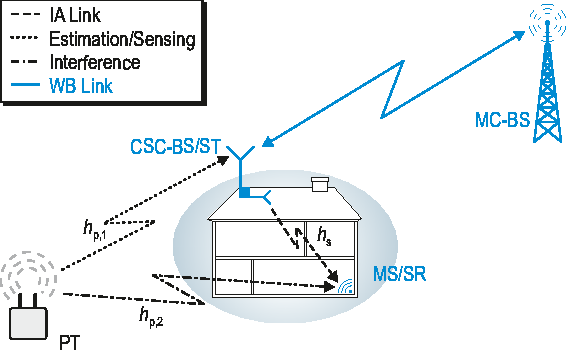
\includegraphics[width = 0.45 \columnwidth]{figures/CR_Scenario_Interweave5} \quad 
\label{fig:CSC_PCI}} 
\hfil
\subfloat[]{\includegraphics[width = 0.45 \columnwidth]{figures/CR_Scenario_Underlay_gruen}
\label{fig:CSC_PCU}} \\
\subfloat[]{\includegraphics[width = 0.45 \columnwidth]{figures/Frame_Structure_grau_I} \quad
\label{fig:CSC_FSI}}
\hfil
\subfloat[]{\includegraphics[width = 0.45 \columnwidth]{figures/Frame_Structure_grau_U}
\label{fig:CSC_FSU}} 
\caption{An illustration of the deployment scenarios of CSC as IS (a) and US (b) depicting the interaction between the PU (PT or PR), the CSC-BS and the MS. Moreover, the CSC-BS as IS or US employs PTA or PRA as coordination strategy, respectively. (c) and (d) present their corresponding frame structures that include the estimation of the received power, where $\test$, $\tsen$ and $T$ represents the respective time intervals for estimation, sensing and frame duration.}
\label{fig:CSC_R}
\end{figure*}
\subsubsection*{Estimation (Noise)}
With the introduction of the estimation at the ST,
%\begin{itemize}
%\item 
a certain distortion is induced in the system. This distortion, if not considered in the system model, leads to harmful interference at the PR. 
%\item 
%Moreover, the performance in terms of throughput at SU differs from its ideal behaviour. %Hence, this deviation of throughput from its ideal behavior is depicted via a proper choice of the estimation duration depicts this deviation of the throughput from its ideal case. 
%\end{itemize}
The severity in distortion is characterized based on the probability of confidence ($\pc$) and the estimation time. Particularly, it is important to select the estimation time appropriately so that the distortion is sustained below a certain level. Consequently, the estimation time causes the throughput to deviate from its ideal case. The ideal case illustrates the exclusion of the received power estimation from the system. 

Hence, from the deployment perspective, it is essential to include these ingredients in the model. Subsequently, we employ the deployment model to the aforementioned paradigms and characterize the true performance of the CSC. 
%Given the plethora of contemporary wireless standards that differ in their access mode, duplex mode, frequency range, bandwidth and transmit power \cite{Jondral05}, it is inconsiderate to follow one and monotonous to abide all of these. 

%\begin{table}
%\renewcommand{\arraystretch}{1.3}
%\caption{Illustration of CR Paradigms}
%\label{tb:Para}
%\centering
%%\begin{tabular}{b{0.2\columnwidth}||b{0.2\columnwidth}||p{0.2\columnwidth}}
%\begin{tabular}{c||c||c}
%\hline
%& \bfseries Interweave System & \bfseries Underlay System \\
%\hline\hline
%Assistance Strategy & PTA & PRA, PTA \\ \hline
%%Constraint & Probability of detection &  Interference temperature \\ \hline
%Interference Management & Spectrum Sensing &  Power Control \\ \hline
%Performance Parameter (PU) & Probability of detection  &  Interference Temperature \\ \hline
%Performance Parameter (SU) & \makecell{ Throughput \\ (Probability of false alarm, \\ Estimation time)} &  \makecell{Throughput \\(Estimation time)} \\ \hline
%\end{tabular}
%\end{table}

\begin{table}
\renewcommand{\arraystretch}{1.3}
\caption{Parameters for Numerical Analysis}
\label{tb:Para}
\centering
%\begin{tabular}{b{0.2\columnwidth}||b{0.2\columnwidth}||p{0.2\columnwidth}}
\begin{tabular}{c||c|c}
\hline
\bfseries Parameter & \bfseries {Paradigm} & \bfseries Value \\
\hline\hline
Sampling frequency & US, IS &\SI{1}{MHz} \\ \hline
Frame duration & US, IS & \SI{100}{ms} \\ \hline
Estimation time & US, IS & \SI{10}{ms} \\ \hline
Probability of confidence & US, IS & 0.95 \\ \hline
Noise power (PU, ST, SR) & US, IS &\SI{-100}{dBm} \\ \hline
PU transmit power & US, IS &\SI{0}{dBm} \\ \hline 
Channel gain ($\hpo,\hpt$) & IS & \SI{-100}{dB} \\ \hline
Channel gain ($\hp$) & US &\SI{-100}{dB} \\ \hline
Channel gain ($\hs$)  & US, IS & \SI{-80}{dB} \\ \hline
PU Channel occupancy & IS & 20\% \\ \hline
Interference threshold & US & \SI{-110}{dBm}
\end{tabular}
\end{table}


%%%%%%%%%%%%%%%%%%%%%%%%%%%%%%%%%%%%%%%%%%%%%%%%%%%%%%%%%%%%%%%%%%%%%%%%%%%%%%%%%%%%%%%%%
\section{CSC as Interweave System} \label{sec:para_i}
%%%%%%%%%%%%%%%%%%%%%%%%%%%%%%%%%%%%%%%%%%%%%%%%%%%%%%%%%%%%%%%%%%%%%%%%%%%%%%%%%%%%%%%%%
The CSC-BS as IS employs sensing to determine the presence or absence of the primary signal in time, frequency and space domains. Although, several techniques such as energy detection, matched filtering, cyclostationary and feature-based detection exist, energy detection is widely investigated in the literature due to its versatility towards unknown primary signals. Hereby, the ST performs hypothesis testing by listening to the transmission from the PT. Subsequently, the received power is compared to a detection threshold. This way, the ST is able to protect the PR against interference. Based on this discussion, for IS, it is reasonable to employ PTA at the ST, cf. \figurename~\ref{fig:CSC_PCI}. 

The probability of detection ($\pd$) and probability of false alarm ($\pf$) characterize the performance of the system. To ensure an interference-free transmission, the ST must sustain a minimum level of $\pd$. With the knowledge of the received power, it is feasible to determine an optimum sensing time and the detection threshold \cite{Liang08}. Considering a hardware deployment, this knowledge however is not available at the ST. In this regard, we propose a new frame structure, cf. \figurename~\ref{fig:CSC_FSI}, that includes the received power estimation \cite{Kaushik15_CC}. The estimation is followed by the sensing and the data transmission. 

Next, we investigate the effect of estimation on the performance of the IS.
The distortion in the system is captured by defining the maximum and minimum value of the estimated received power characterized in terms of a confidence interval. This confidence interval is determined for a certain choice of $\pc$. Whereby, these intervals lead to distortion in the optimum sensing and the detection threshold that finally translate to distortion in the performance parameters, i.e., $\pd$ and throughput. 
 \figurename~{\ref{fig:PP_I_pd}} presents the distortion in $\pd$ (by means of upper and lower bounds) versus the estimation time for different values of received Signal to Noise Ratio (SNR) at the ST, where $\pd = 0.9$ is desired. 
It is worth noticing that the distortion becomes intolerable for low values and negligible for high values of received SNR. \figurename~{\ref{fig:PP_I_th}} depicts the optimum throughput (optimized over the sensing time) versus received SNR, where the estimation time equals \SI{10}{ms}. The case with $\pc = 0$ illustrates a situation under which the estimation of the received power is included in the system, however, it is perfect. Besides that, \figurename~{\ref{fig:PP_I_th}} depicts the deviation in the optimum throughput from the ideal case (with no estimation). 
%Again it is reflected from \figurename~{\ref{fig:PP_I_th}} that low received SNR will result in large distortion in the optimum throughput. 
Hence, based on this characterization, it is feasible to define an operation regime of the CSC-BS in terms of the received SNR by selecting the $\pc$ and estimation time appropriately. 
\begin{figure}[!t]
\centering
%% Add psfrag entries
%\caption{The figure captures the distortion in probability of detection versus the estimation time for different received SNR $\in \{-10,-5,0, \infty\}\SI{}{dB}$ \cite{Kaushik15_CC}.}
%\label{fig:pd_test}
%\end{figure}
%\begin{figure}[!t]
%\centering
%% Add psfrag entries
%\hfil
\subfloat[]{
	% This file is generated by the MATLAB m-file laprint.m. It can be included
% into LaTeX documents using the packages graphicx, color and psfrag.
% It is accompanied by a postscript file. A sample LaTeX file is:
%    \documentclass{article}\usepackage{graphicx,color,psfrag}
%    \begin{document}% This file is generated by the MATLAB m-file laprint.m. It can be included
% into LaTeX documents using the packages graphicx, color and psfrag.
% It is accompanied by a postscript file. A sample LaTeX file is:
%    \documentclass{article}\usepackage{graphicx,color,psfrag}
%    \begin{document}% This file is generated by the MATLAB m-file laprint.m. It can be included
% into LaTeX documents using the packages graphicx, color and psfrag.
% It is accompanied by a postscript file. A sample LaTeX file is:
%    \documentclass{article}\usepackage{graphicx,color,psfrag}
%    \begin{document}\input{fig_P_d_vs_est_time_diff_snr_AWGN_ComMag}\end{document}
% See http://www.mathworks.de/matlabcentral/fileexchange/loadFile.do?objectId=4638
% for recent versions of laprint.m.
%
% created by:           LaPrint version 3.16 (13.9.2004)
% created on:           23-Feb-2015 08:44:53
% eps bounding box:     14 cm x 10.5 cm
% comment:              
%
%\begin{psfrags}%
%\psfragscanon%
%
% text strings:
\psfrag{s01}[b][b]{\fontsize{7.5}{11.25}\fontseries{m}\mathversion{normal}\fontshape{n}\selectfont \color[rgb]{0,0,0}\setlength{\tabcolsep}{0pt}\begin{tabular}{c}Probability of Detection\end{tabular}}%
\psfrag{s02}[t][t]{\fontsize{7.5}{11.25}\fontseries{m}\mathversion{normal}\fontshape{n}\selectfont \color[rgb]{0,0,0}\setlength{\tabcolsep}{0pt}\begin{tabular}{c}Estimation Time [ms]\end{tabular}}%
\psfrag{s06}[][]{\fontsize{10}{15}\fontseries{m}\mathversion{normal}\fontshape{n}\selectfont \color[rgb]{0,0,0}\setlength{\tabcolsep}{0pt}\begin{tabular}{c} \end{tabular}}%
\psfrag{s07}[][]{\fontsize{10}{15}\fontseries{m}\mathversion{normal}\fontshape{n}\selectfont \color[rgb]{0,0,0}\setlength{\tabcolsep}{0pt}\begin{tabular}{c} \end{tabular}}%
\psfrag{s08}[l][l]{\fontsize{7.5}{11.25}\fontseries{m}\mathversion{normal}\fontshape{n}\selectfont \color[rgb]{0,0,0}SNR = $\infty$ dB}%
\psfrag{s09}[l][l]{\fontsize{7.5}{11.25}\fontseries{m}\mathversion{normal}\fontshape{n}\selectfont \color[rgb]{0,0,0}SNR = \SI{-10}{dB}}%
\psfrag{s10}[l][l]{\fontsize{7.5}{11.25}\fontseries{m}\mathversion{normal}\fontshape{n}\selectfont \color[rgb]{0,0,0}SNR = \SI{-5}{dB}}%
\psfrag{s11}[l][l]{\fontsize{7.5}{11.25}\fontseries{m}\mathversion{normal}\fontshape{n}\selectfont \color[rgb]{0,0,0}SNR = \SI{0}{dB}}%
\psfrag{s12}[l][l]{\fontsize{7.5}{11.25}\fontseries{m}\mathversion{normal}\fontshape{n}\selectfont \color[rgb]{0,0,0}SNR = $\infty$ dB}%
%
% axes font properties:
\fontsize{7.5}{11.25}\fontseries{m}\mathversion{normal}%
\fontshape{n}\selectfont%
%
% xticklabels:
\psfrag{x01}[t][t]{2}%
\psfrag{x02}[t][t]{4}%
\psfrag{x03}[t][t]{6}%
\psfrag{x04}[t][t]{8}%
\psfrag{x05}[t][t]{10}%
\psfrag{x06}[t][t]{12}%
\psfrag{x07}[t][t]{14}%
%
% yticklabels:
\psfrag{v01}[r][r]{0.4}%
\psfrag{v02}[r][r]{0.5}%
\psfrag{v03}[r][r]{0.6}%
\psfrag{v04}[r][r]{0.7}%
\psfrag{v05}[r][r]{0.8}%
\psfrag{v06}[r][r]{0.9}%
\psfrag{v07}[r][r]{1}%
%
% Figure:
%\resizebox{7cm}{!}{\includegraphics{fig_P_d_vs_est_time_diff_snr_AWGN_ComMag.eps}}%
%\end{psfrags}%
%
% End fig_P_d_vs_est_time_diff_snr_AWGN_ComMag.tex
\end{document}
% See http://www.mathworks.de/matlabcentral/fileexchange/loadFile.do?objectId=4638
% for recent versions of laprint.m.
%
% created by:           LaPrint version 3.16 (13.9.2004)
% created on:           23-Feb-2015 08:44:53
% eps bounding box:     14 cm x 10.5 cm
% comment:              
%
%\begin{psfrags}%
%\psfragscanon%
%
% text strings:
\psfrag{s01}[b][b]{\fontsize{7.5}{11.25}\fontseries{m}\mathversion{normal}\fontshape{n}\selectfont \color[rgb]{0,0,0}\setlength{\tabcolsep}{0pt}\begin{tabular}{c}Probability of Detection\end{tabular}}%
\psfrag{s02}[t][t]{\fontsize{7.5}{11.25}\fontseries{m}\mathversion{normal}\fontshape{n}\selectfont \color[rgb]{0,0,0}\setlength{\tabcolsep}{0pt}\begin{tabular}{c}Estimation Time [ms]\end{tabular}}%
\psfrag{s06}[][]{\fontsize{10}{15}\fontseries{m}\mathversion{normal}\fontshape{n}\selectfont \color[rgb]{0,0,0}\setlength{\tabcolsep}{0pt}\begin{tabular}{c} \end{tabular}}%
\psfrag{s07}[][]{\fontsize{10}{15}\fontseries{m}\mathversion{normal}\fontshape{n}\selectfont \color[rgb]{0,0,0}\setlength{\tabcolsep}{0pt}\begin{tabular}{c} \end{tabular}}%
\psfrag{s08}[l][l]{\fontsize{7.5}{11.25}\fontseries{m}\mathversion{normal}\fontshape{n}\selectfont \color[rgb]{0,0,0}SNR = $\infty$ dB}%
\psfrag{s09}[l][l]{\fontsize{7.5}{11.25}\fontseries{m}\mathversion{normal}\fontshape{n}\selectfont \color[rgb]{0,0,0}SNR = \SI{-10}{dB}}%
\psfrag{s10}[l][l]{\fontsize{7.5}{11.25}\fontseries{m}\mathversion{normal}\fontshape{n}\selectfont \color[rgb]{0,0,0}SNR = \SI{-5}{dB}}%
\psfrag{s11}[l][l]{\fontsize{7.5}{11.25}\fontseries{m}\mathversion{normal}\fontshape{n}\selectfont \color[rgb]{0,0,0}SNR = \SI{0}{dB}}%
\psfrag{s12}[l][l]{\fontsize{7.5}{11.25}\fontseries{m}\mathversion{normal}\fontshape{n}\selectfont \color[rgb]{0,0,0}SNR = $\infty$ dB}%
%
% axes font properties:
\fontsize{7.5}{11.25}\fontseries{m}\mathversion{normal}%
\fontshape{n}\selectfont%
%
% xticklabels:
\psfrag{x01}[t][t]{2}%
\psfrag{x02}[t][t]{4}%
\psfrag{x03}[t][t]{6}%
\psfrag{x04}[t][t]{8}%
\psfrag{x05}[t][t]{10}%
\psfrag{x06}[t][t]{12}%
\psfrag{x07}[t][t]{14}%
%
% yticklabels:
\psfrag{v01}[r][r]{0.4}%
\psfrag{v02}[r][r]{0.5}%
\psfrag{v03}[r][r]{0.6}%
\psfrag{v04}[r][r]{0.7}%
\psfrag{v05}[r][r]{0.8}%
\psfrag{v06}[r][r]{0.9}%
\psfrag{v07}[r][r]{1}%
%
% Figure:
%\resizebox{7cm}{!}{\includegraphics{fig_P_d_vs_est_time_diff_snr_AWGN_ComMag.eps}}%
%\end{psfrags}%
%
% End fig_P_d_vs_est_time_diff_snr_AWGN_ComMag.tex
\end{document}
% See http://www.mathworks.de/matlabcentral/fileexchange/loadFile.do?objectId=4638
% for recent versions of laprint.m.
%
% created by:           LaPrint version 3.16 (13.9.2004)
% created on:           23-Feb-2015 08:44:53
% eps bounding box:     14 cm x 10.5 cm
% comment:              
%
%\begin{psfrags}%
%\psfragscanon%
%
% text strings:
\psfrag{s01}[b][b]{\fontsize{7.5}{11.25}\fontseries{m}\mathversion{normal}\fontshape{n}\selectfont \color[rgb]{0,0,0}\setlength{\tabcolsep}{0pt}\begin{tabular}{c}Probability of Detection\end{tabular}}%
\psfrag{s02}[t][t]{\fontsize{7.5}{11.25}\fontseries{m}\mathversion{normal}\fontshape{n}\selectfont \color[rgb]{0,0,0}\setlength{\tabcolsep}{0pt}\begin{tabular}{c}Estimation Time [ms]\end{tabular}}%
\psfrag{s06}[][]{\fontsize{10}{15}\fontseries{m}\mathversion{normal}\fontshape{n}\selectfont \color[rgb]{0,0,0}\setlength{\tabcolsep}{0pt}\begin{tabular}{c} \end{tabular}}%
\psfrag{s07}[][]{\fontsize{10}{15}\fontseries{m}\mathversion{normal}\fontshape{n}\selectfont \color[rgb]{0,0,0}\setlength{\tabcolsep}{0pt}\begin{tabular}{c} \end{tabular}}%
\psfrag{s08}[l][l]{\fontsize{7.5}{11.25}\fontseries{m}\mathversion{normal}\fontshape{n}\selectfont \color[rgb]{0,0,0}SNR = $\infty$ dB}%
\psfrag{s09}[l][l]{\fontsize{7.5}{11.25}\fontseries{m}\mathversion{normal}\fontshape{n}\selectfont \color[rgb]{0,0,0}SNR = \SI{-10}{dB}}%
\psfrag{s10}[l][l]{\fontsize{7.5}{11.25}\fontseries{m}\mathversion{normal}\fontshape{n}\selectfont \color[rgb]{0,0,0}SNR = \SI{-5}{dB}}%
\psfrag{s11}[l][l]{\fontsize{7.5}{11.25}\fontseries{m}\mathversion{normal}\fontshape{n}\selectfont \color[rgb]{0,0,0}SNR = \SI{0}{dB}}%
\psfrag{s12}[l][l]{\fontsize{7.5}{11.25}\fontseries{m}\mathversion{normal}\fontshape{n}\selectfont \color[rgb]{0,0,0}SNR = $\infty$ dB}%
%
% axes font properties:
\fontsize{7.5}{11.25}\fontseries{m}\mathversion{normal}%
\fontshape{n}\selectfont%
%
% xticklabels:
\psfrag{x01}[t][t]{2}%
\psfrag{x02}[t][t]{4}%
\psfrag{x03}[t][t]{6}%
\psfrag{x04}[t][t]{8}%
\psfrag{x05}[t][t]{10}%
\psfrag{x06}[t][t]{12}%
\psfrag{x07}[t][t]{14}%
%
% yticklabels:
\psfrag{v01}[r][r]{0.4}%
\psfrag{v02}[r][r]{0.5}%
\psfrag{v03}[r][r]{0.6}%
\psfrag{v04}[r][r]{0.7}%
\psfrag{v05}[r][r]{0.8}%
\psfrag{v06}[r][r]{0.9}%
\psfrag{v07}[r][r]{1}%
%
% Figure:
%\resizebox{7cm}{!}{\includegraphics{fig_P_d_vs_est_time_diff_snr_AWGN_ComMag.eps}}%
%\end{psfrags}%
%
% End fig_P_d_vs_est_time_diff_snr_AWGN_ComMag.tex


        \begin{tikzpicture}[scale=1]
                \node[anchor=south west,inner sep=0] (image) at (0,0)
                {  
			\includegraphics[width=0.47\columnwidth]{figures/fig_P_d_vs_est_time_diff_snr_AWGN_ComMag}
                };
                \begin{scope}[x={(image.south east)},y={(image.north west)}]

                % Select curves depending upon theta  
                \draw (0.29,0.89) arc(-180:180:1.00mm and 3.50mm);
                \node[draw,fill=gray!10,font=\scriptsize] (UB) at (0.2,0.69) {Upper Bound};
                \draw[black, dashed] (UB.north) -- (0.304,0.833);
                
                \draw (0.8,0.67) arc(-180:180:2.20mm and 7.70mm);
                \node[draw,fill=gray!10,font=\scriptsize] (LB) at (0.65,0.32) {Lower Bound};
                \draw[black, dashed] (LB.north) -- (0.83,0.55);
 

                %\draw[help lines,xstep=.1,ystep=.1] (0,0) grid (1,1);
                %\foreach \x in {0,1,...,9} { \node [anchor=north] at (\x/10,0) {0.\x}; }
                %\foreach \y in {0,1,...,9} { \node [anchor=east] at (0,\y/10) {0.\y}; }
                \end{scope}
        \end{tikzpicture}

\label{fig:PP_I_pd}
}
\hfil
\subfloat[]{
	% This file is generated by the MATLAB m-file laprint.m. It can be included
% into LaTeX documents using the packages graphicx, color and psfrag.
% It is accompanied by a postscript file. A sample LaTeX file is:
%    \documentclass{article}\usepackage{graphicx,color,psfrag}
%    \begin{document}% This file is generated by the MATLAB m-file laprint.m. It can be included
% into LaTeX documents using the packages graphicx, color and psfrag.
% It is accompanied by a postscript file. A sample LaTeX file is:
%    \documentclass{article}\usepackage{graphicx,color,psfrag}
%    \begin{document}% This file is generated by the MATLAB m-file laprint.m. It can be included
% into LaTeX documents using the packages graphicx, color and psfrag.
% It is accompanied by a postscript file. A sample LaTeX file is:
%    \documentclass{article}\usepackage{graphicx,color,psfrag}
%    \begin{document}\input{fig_opt_thr_vs_SNR_AWGN_10_ComMag}\end{document}
% See http://www.mathworks.de/matlabcentral/fileexchange/loadFile.do?objectId=4638
% for recent versions of laprint.m.
%
% created by:           LaPrint version 3.16 (13.9.2004)
% created on:           23-Feb-2015 08:47:40
% eps bounding box:     14 cm x 10.5 cm
% comment:              
%
%\begin{psfrags}%
%\psfragscanon%
%
% text strings:
\psfrag{s01}[b][b]{\fontsize{7.5}{11.25}\fontseries{m}\mathversion{normal}\fontshape{n}\selectfont \color[rgb]{0,0,0}\setlength{\tabcolsep}{0pt}\begin{tabular}{c}Throughput at SR [bits/sec/Hz]\end{tabular}}%
\psfrag{s02}[t][t]{\fontsize{7.5}{11.25}\fontseries{m}\mathversion{normal}\fontshape{n}\selectfont \color[rgb]{0,0,0}\setlength{\tabcolsep}{0pt}\begin{tabular}{c}$\snrrcvd$ [dB]\end{tabular}}%
\psfrag{s06}[][]{\fontsize{10}{15}\fontseries{m}\mathversion{normal}\fontshape{n}\selectfont \color[rgb]{0,0,0}\setlength{\tabcolsep}{0pt}\begin{tabular}{c} \end{tabular}}%
\psfrag{s07}[][]{\fontsize{10}{15}\fontseries{m}\mathversion{normal}\fontshape{n}\selectfont \color[rgb]{0,0,0}\setlength{\tabcolsep}{0pt}\begin{tabular}{c} \end{tabular}}%
\psfrag{s08}[l][l]{\fontsize{7.5}{11.25}\fontseries{m}\mathversion{normal}\fontshape{n}\selectfont \color[rgb]{0,0,0}$\pc = 0.97$}%
\psfrag{s09}[l][l]{\fontsize{7.5}{11.25}\fontseries{m}\mathversion{normal}\fontshape{n}\selectfont \color[rgb]{0,0,0}Ideal Case}%
\psfrag{s10}[l][l]{\fontsize{7.5}{11.25}\fontseries{m}\mathversion{normal}\fontshape{n}\selectfont \color[rgb]{0,0,0}$\pc = 0$}%
\psfrag{s11}[l][l]{\fontsize{7.5}{11.25}\fontseries{m}\mathversion{normal}\fontshape{n}\selectfont \color[rgb]{0,0,0}$\pc = 0.92$}%
\psfrag{s12}[l][l]{\fontsize{7.5}{11.25}\fontseries{m}\mathversion{normal}\fontshape{n}\selectfont \color[rgb]{0,0,0}$\pc = 0.95$}%
\psfrag{s13}[l][l]{\fontsize{7.5}{11.25}\fontseries{m}\mathversion{normal}\fontshape{n}\selectfont \color[rgb]{0,0,0}$\pc = 0.97$}%
%
% axes font properties:
\fontsize{7.5}{11.25}\fontseries{m}\mathversion{normal}%
\fontshape{n}\selectfont%
%
% xticklabels:
\psfrag{x01}[t][t]{-10}%
\psfrag{x02}[t][t]{-5}%
\psfrag{x03}[t][t]{0}%
\psfrag{x04}[t][t]{5}%
\psfrag{x05}[t][t]{10}%
%
% yticklabels:
\psfrag{v01}[r][r]{1}%
\psfrag{v02}[r][r]{1.5}%
\psfrag{v03}[r][r]{2}%
\psfrag{v04}[r][r]{2.5}%
%
% Figure:
%\resizebox{7cm}{!}{\includegraphics{fig_opt_thr_vs_SNR_AWGN_10_ComMag.eps}}%
%\end{psfrags}%
%
% End fig_opt_thr_vs_SNR_AWGN_10_ComMag.tex
\end{document}
% See http://www.mathworks.de/matlabcentral/fileexchange/loadFile.do?objectId=4638
% for recent versions of laprint.m.
%
% created by:           LaPrint version 3.16 (13.9.2004)
% created on:           23-Feb-2015 08:47:40
% eps bounding box:     14 cm x 10.5 cm
% comment:              
%
%\begin{psfrags}%
%\psfragscanon%
%
% text strings:
\psfrag{s01}[b][b]{\fontsize{7.5}{11.25}\fontseries{m}\mathversion{normal}\fontshape{n}\selectfont \color[rgb]{0,0,0}\setlength{\tabcolsep}{0pt}\begin{tabular}{c}Throughput at SR [bits/sec/Hz]\end{tabular}}%
\psfrag{s02}[t][t]{\fontsize{7.5}{11.25}\fontseries{m}\mathversion{normal}\fontshape{n}\selectfont \color[rgb]{0,0,0}\setlength{\tabcolsep}{0pt}\begin{tabular}{c}$\snrrcvd$ [dB]\end{tabular}}%
\psfrag{s06}[][]{\fontsize{10}{15}\fontseries{m}\mathversion{normal}\fontshape{n}\selectfont \color[rgb]{0,0,0}\setlength{\tabcolsep}{0pt}\begin{tabular}{c} \end{tabular}}%
\psfrag{s07}[][]{\fontsize{10}{15}\fontseries{m}\mathversion{normal}\fontshape{n}\selectfont \color[rgb]{0,0,0}\setlength{\tabcolsep}{0pt}\begin{tabular}{c} \end{tabular}}%
\psfrag{s08}[l][l]{\fontsize{7.5}{11.25}\fontseries{m}\mathversion{normal}\fontshape{n}\selectfont \color[rgb]{0,0,0}$\pc = 0.97$}%
\psfrag{s09}[l][l]{\fontsize{7.5}{11.25}\fontseries{m}\mathversion{normal}\fontshape{n}\selectfont \color[rgb]{0,0,0}Ideal Case}%
\psfrag{s10}[l][l]{\fontsize{7.5}{11.25}\fontseries{m}\mathversion{normal}\fontshape{n}\selectfont \color[rgb]{0,0,0}$\pc = 0$}%
\psfrag{s11}[l][l]{\fontsize{7.5}{11.25}\fontseries{m}\mathversion{normal}\fontshape{n}\selectfont \color[rgb]{0,0,0}$\pc = 0.92$}%
\psfrag{s12}[l][l]{\fontsize{7.5}{11.25}\fontseries{m}\mathversion{normal}\fontshape{n}\selectfont \color[rgb]{0,0,0}$\pc = 0.95$}%
\psfrag{s13}[l][l]{\fontsize{7.5}{11.25}\fontseries{m}\mathversion{normal}\fontshape{n}\selectfont \color[rgb]{0,0,0}$\pc = 0.97$}%
%
% axes font properties:
\fontsize{7.5}{11.25}\fontseries{m}\mathversion{normal}%
\fontshape{n}\selectfont%
%
% xticklabels:
\psfrag{x01}[t][t]{-10}%
\psfrag{x02}[t][t]{-5}%
\psfrag{x03}[t][t]{0}%
\psfrag{x04}[t][t]{5}%
\psfrag{x05}[t][t]{10}%
%
% yticklabels:
\psfrag{v01}[r][r]{1}%
\psfrag{v02}[r][r]{1.5}%
\psfrag{v03}[r][r]{2}%
\psfrag{v04}[r][r]{2.5}%
%
% Figure:
%\resizebox{7cm}{!}{\includegraphics{fig_opt_thr_vs_SNR_AWGN_10_ComMag.eps}}%
%\end{psfrags}%
%
% End fig_opt_thr_vs_SNR_AWGN_10_ComMag.tex
\end{document}
% See http://www.mathworks.de/matlabcentral/fileexchange/loadFile.do?objectId=4638
% for recent versions of laprint.m.
%
% created by:           LaPrint version 3.16 (13.9.2004)
% created on:           23-Feb-2015 08:47:40
% eps bounding box:     14 cm x 10.5 cm
% comment:              
%
%\begin{psfrags}%
%\psfragscanon%
%
% text strings:
\psfrag{s01}[b][b]{\fontsize{7.5}{11.25}\fontseries{m}\mathversion{normal}\fontshape{n}\selectfont \color[rgb]{0,0,0}\setlength{\tabcolsep}{0pt}\begin{tabular}{c}Throughput at SR [bits/sec/Hz]\end{tabular}}%
\psfrag{s02}[t][t]{\fontsize{7.5}{11.25}\fontseries{m}\mathversion{normal}\fontshape{n}\selectfont \color[rgb]{0,0,0}\setlength{\tabcolsep}{0pt}\begin{tabular}{c}$\snrrcvd$ [dB]\end{tabular}}%
\psfrag{s06}[][]{\fontsize{10}{15}\fontseries{m}\mathversion{normal}\fontshape{n}\selectfont \color[rgb]{0,0,0}\setlength{\tabcolsep}{0pt}\begin{tabular}{c} \end{tabular}}%
\psfrag{s07}[][]{\fontsize{10}{15}\fontseries{m}\mathversion{normal}\fontshape{n}\selectfont \color[rgb]{0,0,0}\setlength{\tabcolsep}{0pt}\begin{tabular}{c} \end{tabular}}%
\psfrag{s08}[l][l]{\fontsize{7.5}{11.25}\fontseries{m}\mathversion{normal}\fontshape{n}\selectfont \color[rgb]{0,0,0}$\pc = 0.97$}%
\psfrag{s09}[l][l]{\fontsize{7.5}{11.25}\fontseries{m}\mathversion{normal}\fontshape{n}\selectfont \color[rgb]{0,0,0}Ideal Case}%
\psfrag{s10}[l][l]{\fontsize{7.5}{11.25}\fontseries{m}\mathversion{normal}\fontshape{n}\selectfont \color[rgb]{0,0,0}$\pc = 0$}%
\psfrag{s11}[l][l]{\fontsize{7.5}{11.25}\fontseries{m}\mathversion{normal}\fontshape{n}\selectfont \color[rgb]{0,0,0}$\pc = 0.92$}%
\psfrag{s12}[l][l]{\fontsize{7.5}{11.25}\fontseries{m}\mathversion{normal}\fontshape{n}\selectfont \color[rgb]{0,0,0}$\pc = 0.95$}%
\psfrag{s13}[l][l]{\fontsize{7.5}{11.25}\fontseries{m}\mathversion{normal}\fontshape{n}\selectfont \color[rgb]{0,0,0}$\pc = 0.97$}%
%
% axes font properties:
\fontsize{7.5}{11.25}\fontseries{m}\mathversion{normal}%
\fontshape{n}\selectfont%
%
% xticklabels:
\psfrag{x01}[t][t]{-10}%
\psfrag{x02}[t][t]{-5}%
\psfrag{x03}[t][t]{0}%
\psfrag{x04}[t][t]{5}%
\psfrag{x05}[t][t]{10}%
%
% yticklabels:
\psfrag{v01}[r][r]{1}%
\psfrag{v02}[r][r]{1.5}%
\psfrag{v03}[r][r]{2}%
\psfrag{v04}[r][r]{2.5}%
%
% Figure:
%\resizebox{7cm}{!}{\includegraphics{fig_opt_thr_vs_SNR_AWGN_10_ComMag.eps}}%
%\end{psfrags}%
%
% End fig_opt_thr_vs_SNR_AWGN_10_ComMag.tex

	\begin{tikzpicture}[scale=1]
		\node[anchor=south west,inner sep=0] (image) at (0,0)
		{  
			\includegraphics[width=0.47\columnwidth]{figures/fig_opt_thr_vs_SNR_AWGN_10_ComMag}
		};
		\begin{scope}[x={(image.south east)},y={(image.north west)}]

		% Select curves depending upon theta  
		\draw (0.25,0.87) arc(-180:180:0.70mm and 1.40mm);
		\node[draw,fill=gray!10,font=\scriptsize] (UB) at (0.459,0.647) {Upper Bound};
		\draw[black, dashed] (UB.north) -- (0.259,0.847);
		
		\draw (0.2,0.72) arc(-180:180:0.70mm and 1.40mm);
		\node[draw,fill=gray!10,font=\scriptsize] (LB) at (0.409,0.497) {Lower Bound};
		\draw[black, dashed] (LB.north) -- (0.209,0.697);
 

		%\draw[help lines,xstep=.1,ystep=.1] (0,0) grid (1,1);
		%\foreach \x in {0,1,...,9} { \node [anchor=north] at (\x/10,0) {0.\x}; }
		%\foreach \y in {0,1,...,9} { \node [anchor=east] at (0,\y/10) {0.\y}; }
		\end{scope}
	\end{tikzpicture}
	
\label{fig:PP_I_th}
}
\caption{(a) The distortion in probability of detection versus the estimation time for different received SNR $\in \{-10,-5,0, \infty\}$ \SI{}{dB}. 
(b) The distortion in the optimum throughput at SR versus the received SNR with $\pc \in \{0,0.92,0.95,0.97 \}$, where the estimation time equals \SI{10}{ms} \cite{Kaushik15_CC}.
}
\label{fig:PP_I}
\end{figure}


\subsection*{Proof-of-concept}
Besides characterizing the performance of the system based on analytical expressions, it is equally challenging to depict its hardware realizability. In this belief, we present a hardware demonstrating the feasibility of the CSC-BS as IS, cf. \figurename~\ref{fig:HW_int}. An SDR based platform is utilized to sense multiple non-contiguous GSM \SI{1800}{MHz} downlink channels, the graphical interface is depicted in \figurename~\ref{fig:HW_gui}. In this scenario, the GSM BSs are categorized as PTs. To implement binary hypothesis, the hardware was calibrated. Whereby, \SI{-102}{dBm} was determined as the noise power, in this regard, the detection threshold was set to \SI{-100}{dBm}. A database was installed to access the GSM channel list and to store the binary values corresponding to each channel. With the intention of implementing sensing over the complete downlink spectrum (\SI{1805.2}{MHz} -- \SI{1879.2}{MHz}), we deployed frequency-hopping to perform the sensing over individual channels. A cognitive engine that enables learning based on the channel occupancy is a subject of our ongoing research.  

\begin{figure}[!t]
\centering
\subfloat[]{ \includegraphics[width = 0.7 \columnwidth]{figures/HW_setup} 
\label{fig:HW_int}
} \\
\vfil
\subfloat[]{\includegraphics[width = 0.7 \columnwidth]{figures/Grafik_Poster}
\label{fig:HW_gui}
} 
\caption{(a) A hardware and software architecture of an SDR based demonstrator
depicting the CSC-BS as IS. (b) A snapshot of the Graphical User Interface of the demonstrator, whereby the slices (red and white) represent the channel occupancy (1 or 0) corresponding to a single measurement at a given time instant. The bar plots illustrate the channel occupancy (u) for each channel with a history of 500 measurements.}
\label{fig:HW_I}
\end{figure}

%\begin{itemize}
%	\item Frame Structure
%	\item System model 
%	\item Design parameters: Constraints and performance parameters
%	\item Performance analysis -- Sensing throughput tradeoff
%	\item CSC deployed for indoor scenarios favours the performance of the CSC. As indoor scenarios are prone to high path loss exponent between the CSC and the primary systems -- demonstrate based on the numerical analysis (If possible!) 
%	\item Multiple CSC (Nice to have!)
%\end{itemize}

%%%%%%%%%%%%%%%%%%%%%%%%%%%%%%%%%%%%%%%%%%%%%%%%%%%%%%%%%%%%%%%%%%%%%%%%%%%%%%%%%%%%%%%%%
\section{CSC as Underlay System} \label{sec:para_u}
%%%%%%%%%%%%%%%%%%%%%%%%%%%%%%%%%%%%%%%%%%%%%%%%%%%%%%%%%%%%%%%%%%%%%%%%%%%%%%%%%%%%%%%%%
According to the US, it is permissible for CSC-BS to transmit in the frequency bands where PUs are active, the situation in which PUs are susceptible to a certain level of interference results in better utilization of the spectrum resources. Transmit power control is one such mechanism by which the ST is able to sustain its transmit power below the interference threshold, defined for the PR. Although it is feasible to execute the power control based on either PTA or PRA, however, for the analysis, we apply power control subject to the PRA. 

Now, to execute the power control, the ST needs the knowledge of the channel between the ST and the PR. This information is acquired by listening to a beacon or a pilot channel transmitted by the PR. This way, the ST performs channel estimation based on the received power. As in IS, a new frame structure that includes estimation time followed by data transmission is proposed at the ST, cf. \figurename~\ref{fig:CSC_FSU}. Apparently, limited estimation time leads to variations in the received power, thereby inducing variations in the controlled power at the ST. This causes the power received at the PR to deviate from the interference threshold. Unless investigated, these variations may lead to harmful interference at the PR. Based on $\pc$, we capture these variations in the received power at the PR across the interference threshold. 

Analog to IS, we analyze the effect of estimation on the performance of the US. \figurename~\ref{fig:PP_U_pc} illustrates the dependency of the $\pc$ on the estimation time and received SNR. 
By increasing the estimation time, a certain level of $\pc$ across the interference threshold is acquired. This helps controlling the interference induced due to the estimation. Hence, an appropriate (optimum) choice of estimation time is obligatory for the system. 
%In particular, it is necessary to select the estimation time appropriately to accomplish a desired $\pc = 0.95$. 
For instance, with received SNR = \SI{0}{dB} and $\pc =0.95 $, the optimum estimation time corresponds to $\approx \SI{9.2}{ms}$. \figurename~\ref{fig:PP_U_th} represents the variation of the optimized throughput (optimized over the estimation time) at the SR versus the received SNR for different $\pc$. %, where estimation time is selected optimally. 
Moreover, \figurename~\ref{fig:PP_U_th} depicts a margin between the ideal case (with no estimation) and the deployment model, this margin increases with decrease in received SNR. Based on the analysis, it is worthy to note that the ideal case overestimates the performance, hence, it does not characterize the true performance of the US. 
%\begin{itemize}
%       \item Frame Structure
%       \item System model 
%       \item Design parameters: Constraints and performance parameters
%       \item Performance analysis -- Estimation-throughput tradeoff
%       \item Multiple CSC (Nice to have!)
%       \item CSC deployed for indoor scenarios favours the performance of the CSC. As indoor scenarios are prone to high path loss exponent between the CSC and the primary systems -- demonstrate based on the numerical analysis (If possible!) 
%\end{itemize}
\begin{figure}[!t]
%% Add psfrag entries
%\caption{An illustration of the dependency of the received SNR at CSC-BS on the maximum expected throughput at the CSC-BS for different values of probability of confidence $\pc \in \{0.92, 0.95, 0.97\}$ \cite{Kaushik15}.}
%\label{fig:TvSNR_pl}
%\end{figure}
%\begin{figure}[!t]
%\centering
%% Add psfrag entries
\subfloat[]
{
\input{figures/fig_thr_est_time_tradeoff_AWGN_ComMag.tex}
\label{fig:PP_U_pc}
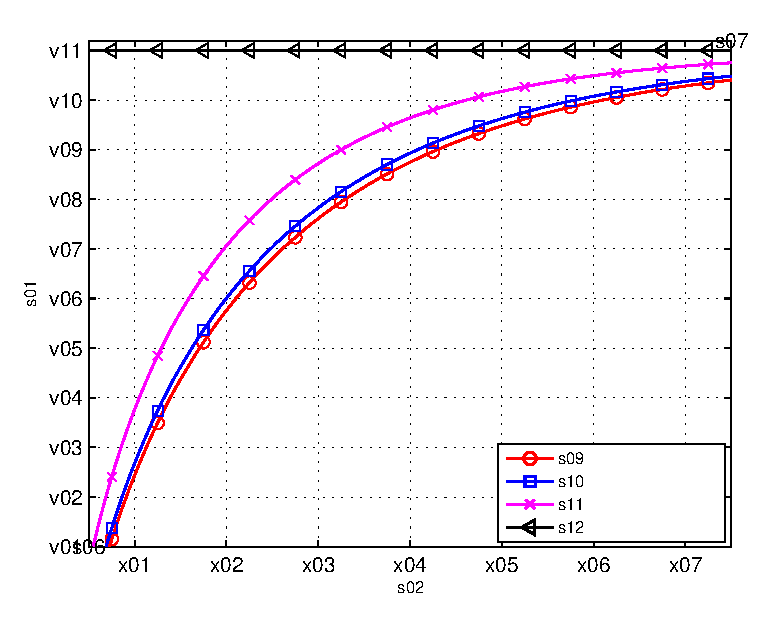
\includegraphics[width=0.47\columnwidth]{figures/fig_thr_est_time_tradeoff_AWGN_ComMag.eps} 
}
\hfil
\subfloat[]{
\input{figures/fig_opt_thr_vs_snr_AWGN_ComMag.tex}
\includegraphics[width=0.47\columnwidth]{figures/fig_opt_thr_vs_snr_AWGN_ComMag}
\label{fig:PP_U_th}
}
\caption{
(a) The $\pc$ versus the estimation time for different received SNR $\in \{-10,-5,0, \infty\}$ \SI{}{dB}. %The $\pc$ captures the severity of distortion in the power received at PR. 
(b) The distortion in the optimum throughput at the SR versus received SNR for different $\pc \in \{0.92, 0.95, 0.97\}$ \cite{Kaushik15}.}
\label{fig:PP_U}
\end{figure}

\subsection*{Proof-of-concept}
In contrast to the theoretical analysis, we briefly illustrate the realizability of the underlay paradigm. In this belief, the hardware feasibility of the US is outlined in \cite{Kaushik14}, whereby the major challenges involved while building a prototype are investigated. An SDR based platform is installed to depict the variations in the propagation channel ($\hp, \hs$), cf. \figurename~\ref{fig:CSC_PCU}. These variations, subject to the mobility of the PR and the MS, are captured and validated based on the analytical expressions. For simplification, a constant transmit power is considered at the CSC-BS. However, it will be interesting to demonstrate the power control mechanism over an SDR based platform. 

%%%%%%%%%%%%%%%%%%%%%%%%%%%%%%%%%%%%%%%%%%%%%%%%%%%%%%%%%%%%%%%%%%%%%%%%%%%%%%%%%%%%%%%%%
\section{Overview of Key Challenges}\label{sec:r_cha} 
%%%%%%%%%%%%%%%%%%%%%%%%%%%%%%%%%%%%%%%%%%%%%%%%%%%%%%%%%%%%%%%%%%%%%%%%%%%%%%%%%%%%%%%%%

In this section, we briefly discuss some of the major key challenges that are subjects of future research. %The estimation model presents the distortion in terms of the received power and rest of the parameters such noise power,  
\subsubsection*{Network-Centric Interference Management}
In this article, we investigated the performance of CSC based on a single CSC-BS and a PU. The interference from the neighbouring CSC-BSs and PUs was excluded in the analysis. Therefore, to characterize the interference in the network, stochastic geometry is currently employed for modelling the locations of the primary (PT, PR) and secondary systems (CSC-BS, MS) \cite{Elsawy13}. Thereby, depicting the performance of CSC based on the stochastic geometry for the CR paradigms poses an interesting research direction. 

%\subsubsection*{Quality of Service (QoS) for CSC}
%The throughput, an important performance parameter, characterizes the QoS inside the CSC. Now, to decide upon the channels in the database subject to a certain QoS, it is essential to evaluate the throughput at the CSC-BS. In this regard, it is necessary to estimate: $\hpt, \hs$ for the IS and; $\hs$ for the US at the MS, and feed back to CSC-BS through a reverse channel. Therefore, characterizing the distortion induced due to the estimation at the MS presents an interesting problem. 

%\subsubsection*{RF Distortions}
%One possible way of extending the deployment model is by incorporating the effect of distortions arising from the RF components. Considering this aspect will lead to a potential enhancement in the performance characterization of the CSC. This could establish a broader perspective and a greater implication on the realizability of the CR technology.  

 
\subsubsection*{Hybrid Techniques}
With the introduction of hybrid techniques, the performance of the system can be improved. These techniques can be illustrated by means of: 
\begin{enumerate}
\item a hybrid coordination strategy, thereby including the assistance from both the PT and the PR; 
\item a hybrid CR paradigm that combines the sensing and transmit power control at the CSC-BS. 
\end{enumerate}

\subsubsection*{Long-Term Policy}
For the analysis, in this article we characterized the performance subject to a single frame, that represents a short-term policy for the CSC. In this regard, we optimized the performance for each frame, thus, the estimation of the system parameter is incorporated within the frame duration. However, one can investigate a long-term policy, which includes a joint estimation of the system parameter preceded by performance optimization across several frames. 
%Lastly, it is noteworthy to consider the duplex mode for the CSC-BS and MS. To proceed further, we consider that likewise, CSC-BS the respective paradigms are employed at the MS. Apart from the conventional signalling information, the CSC-BS and the MS needs to relay additional information such as the current choice of the channel for data transmission. This exchange may happen over a dedicated pilot channel for the IA link. Time division duplexing imposes the devices to share information such as sensing to decide upon a channel, hence, devising a protocol based on this notion presents a challenging task. On the contrary, the frequency division duplexing, that drive the devices to select different channels independently, portrays a relatively simpler solution. 
%\begin{itemize}
%\item Background noise
%\item Interference from the neighbouring CSCs.
%\item Perfect knowledge of the noise power.
%\item In order to accomplish low latency with the CSC, a frequency translation represents a viable solution.
%\item Who will bear the operation expenditure (OPEX): premises owner or mobile operator. 
%\item Infrastructure sharing: One big question is who will pay for the infrastructure and the cost: the users themselves, the mobile operator or will be shared by many operators. This question is dependent on the authority who is willing to pay for it. 
%\item Frequency translation capability -- Wireless backhaul link works on a different frequency compared to the frequency of channels serving indoor devices.  
%\item Considering massive MIMO at the CR to improve energy efficiency and reduce co-tier.
%\item Medium access control between the CSC-BS and MS will be a challenging task.  
%\item Provision for a hybrid paradigm that incorporate spectrum sensing and power control. 
%\item Multiple CSC.
%\end{itemize}
%%%%%%%%%%%%%%%%%%%%%%%%%%%%%%%%%%%%%%%%%%%%%%%%%%%%%%%%%%%%%%%%%%%%%%%%%%%%%%%%%%%%%%%%%
\section{Conclusion} \label{sec:conc}
%%%%%%%%%%%%%%%%%%%%%%%%%%%%%%%%%%%%%%%%%%%%%%%%%%%%%%%%%%%%%%%%%%%%%%%%%%%%%%%%%%%%%%%%%
%Contributing to the 5G evolution is an exciting moment for communication engineers. 

In this article, we have presented a notion of CSC from the deployment perspective. In particular, we have motivated that CSC entails the credibility of overcoming the requirements for the next generation wireless systems. In this context, a preliminary network architecture that considers a successful disposition of the CSC has been presented. We have introduced a novel model that facilitates the deployment of opportunistic access within CSC. For the proposed model, we have specified the key-issues, posed several challenges, and discussed their possible solutions. As an outcome of the analysis, we have emphasized that the existing models, illustrating an ideal scenario, do not characterize the true performance of the CR paradigms. The feasibility of the respective paradigms has been supported with hardware implementations. More importantly, to extend the implications of this concept, we have briefly outlined several open problems and suggested future research directions.     

%Contributing to the 5G evolution is an exciting moment for communication engineers. 
%In the present situation, we are scrutinizing the potential candidates that might lay the foundations of 5G systems. 
%The ultra-densification and the spectrum extension, constituting the largest portion of the desired areal efficiency, are crucial for the 5G systems. However, high deployment costs and the limited spectrum remain the main challenges that hinder the deployment of SCs. %At this moment, we should start orienting ourselves towards flexible cognitive radio solutions to overcome the existing scarcity in the spectrum. 
%Driven by this fact, we proposed the concept of CSC that resolves these challenges to facilitate a technology expansion. This article has motivated the credibility of the CSC to accomplish the requirements for the next generation of wireless systems. %Hence, the deployment of CSC is envisioned as an important ingredient to 5G technology that has the potential of contributing to spectrum requirements. 
%In order to illustrate the feasibility of the opportunistic access at the CSC, we investigated the performance of the underlay and interweave paradigms based on the deployment model. The notion of the CSC poses many interesting challenges as well potential implications on the future of wireless systems. 

%%%%%%%%%%%%%%%%%%%%%%%%%%%%%%%%%%%%%%%%%%%%%%%%%%%%%%%%%%%%%%%%%%%%%%%%%%%%%%%%%%%%%%%%%
% References
%%%%%%%%%%%%%%%%%%%%%%%%%%%%%%%%%%%%%%%%%%%%%%%%%%%%%%%%%%%%%%%%%%%%%%%%%%%%%%%%%%%%%%%%%
\bibliographystyle{IEEEtran}
\bibliography{IEEEabrv,refs}

% that's all from my side
\end{document}
